% Basic LaTeX template for NE 204 lab report
\documentclass[11pt]{article}

%==============================================================================
%%% Everything between the "="'s is the preamble.
%%% Define packages and meta data here

% Common packages
\usepackage{amsmath}    % Expanded math
\usepackage{amssymb}    % Expanded math symbols
\usepackage{graphicx}   % For images
%\usepackage[version=3]{mhchem} % For nuclide formatting

% All images/figures will be stored in the images folder.
% Specify that here so pdflatex knows where to look for images.
\graphicspath{{./images/}}

% Metadata
\title{Calibration Lab report}
\author{Yufei Wang}
\date{\today}
%==============================================================================

\begin{document}

% Compile metadata from preamble into a nicely-rendered title section
\maketitle

% The *'s next so section/subsection definitions suppresses numbering
\section*{Introduction}
\label{sec:intro}
Energy calibration is the very first and important step before using HPGe detectors for radiation detection. A very common way to calibrate is using standard gamma-emitting source, for instance Co-60 and Cs-137. The p-type HPGe with co-axial configuration is used in this experiment and appropriately fitting the date of signal intensity in each energy channel is practiced.


\section*{Methods}
\label{sec:meth}
A group of five isotopes were used to collect the signals, Co-60, Cs-137, Ba-133, Eu-152, and Am-241. The signal intensity (i.e. pulse height) of 8192 channels at different energy ranges were recorded. The MCA would be based upon the characteristic energy of the full energy peaks of the five radionuclides used and linear-regressly correlating the peak centroid to its energy using the least square method. A polinominal form of order 4 to 5 is usually enough. The degree of nonlinearity is often small, so another way to calibrate is plotting deviation from perfect linearity versus channel number. In this report a simple linear regression is seeked.


\[Energy=slope\cdot Channel\,Number + intercept\]

The full energy peak can be fitted as a gaussian curve to get the centroid (B) of each peak:
\[f\left( x \right) = A \cdot {e^{ - \frac{{{{\left( {x - B} \right)}^2}}}{{2 \cdot {C^2}}}}}\]

This is acheived by function $curve\_fit$. Upon obtaining the relationship between the centroid of each peak and the corresponding energy, linear regression using the least square method is adopted to correlate the channel number and the energy range.




\section*{Results}
\label{sec:res}
Major peaks are selected as below with channel v.s. energy in keV:

\begin{table}[h!]
  \begin{center}
    \caption{Peaks with Corresponding Energy.}
    \label{tab:table1}
    \begin{tabular}{l|l|l}
      \textbf{Peak \#} & \textbf{Channel \#} & \textbf{Energy (keV)}\\
      \hline
      1 & 2353.969595281511 & 661.657\\
      2 & 4177.6835240821465 & 1173.228\\
      3 & 4745.511220436352  & 1332.492\\
      4 & 1222.6117121691966  & 344.2785\\
      5 & 1460.7650922753362  & 411.1165\\
      6 & 2772.003206539464  & 778.9045\\
      7 & 3432.077389155436 & 964.072\\
      8 & 5014.927456550307 & 1408.013\\
      9 & 3959.8315489345346 & 1112.076\\
      10 & 980.9088851006587  & 276.3989\\
      11 & 1075.1587761476976 & 302.8508\\
      12 & 1264.6138573728588 & 356.0129\\
      13 & 1363.8190002015974 & 383.8485\\
 
    \end{tabular}
  \end{center}
\end{table}
Linear regression gives
\[Energy[keV]=0.280521278253 \cdot Channel\,Number+1.27621057811\,\,\,\,\,\,\,\,\,(1)\]
with the coefficient of determination being ${R^2}$:
\[{R^2}=0.99999999648747\]
Being close to 1 indicates a good calibration result.




\begin{figure}
  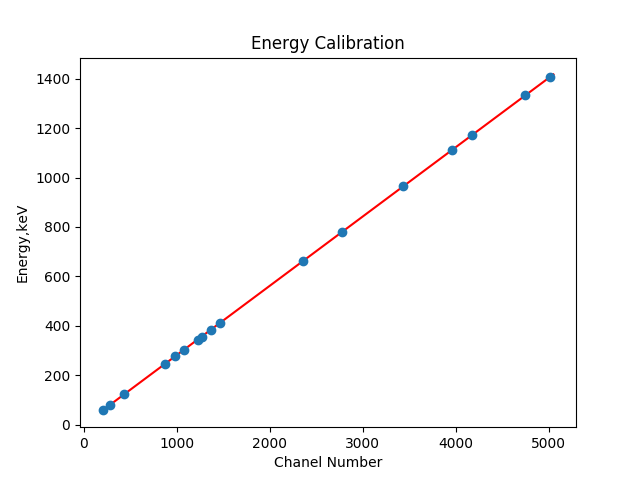
\includegraphics[scale=0.6]{Calibration}
  \caption{Energy Calibration.}
  \label{fig:boat1}
\end{figure}

\section*{Discussion}
\label{sec:disc}
Using part of the five isotopes, one or two, still gives fairly close results. For example, using only Am-241 with a characteristic peak at 59.5409 keV and Cs-137 with a characteristic peak at 661.657 keV gives the following result, which is close to one using all five isotopes:
\[{Energy}=0.2805446 \cdot Channel\,Number+1.263557\,\,\,\,\,\,\,\,\,(2)\]


% Bibliography
\bibliographystyle{plain}
% Refers to a bibtex file in the current dir named "references.bib"
\bibliography{references}

\end{document}
